%#!platex ./report.tex

%
% $BA4BNE*$J>.@a$N$?$F$+$?$,4E$$(B
% $BFbMF$r=q$/=gHV$r9M$($?J}$,$$$$(B

%$B?F$N;^$H$$$&Dj5A$,$o$+$j$K$/$$(B

\chapter{$B8&5f<jK!!&86M}(B}
 \section{$B<jK!$N35MW(B}
   $BK\8&5f$N<jK!$N35N,$O(B, $B$^$:C10l$N?@7P:YK&$,;}$A$&$k5!G=$r$"$i$+$8$a@_Dj$7(B, 
   $B$=$N5!G=$r$&$^$/<B8=$9$k?@7P:YK&7ABV$H%3%s%@%/%?%s%9$NJ,I[$r0dEAE*%"%k%4%j%:%`(B
   $B$rMQ$$$FC5:w$9$k$H$$$&$b$N$G$"$k(B.\cite{torben2009systematic}
   $B?@7P:YK&$N7ABV@8@.$K$O3NN(E*$J<jK!$rMQ$$(B,$B$=$N:]$KMQ$$$k3NN(%Q%i%a!<%?$r(B
   $B0dEAE*%"%k%4%j%:%`$N0dEA;R$H$7$F07$&(B.
 \section{$B?@7P:YK&$N5!G=(B}
   $BK\8&5f$G?@7P:YK&$K@_Dj$9$k5!G=$O(B, $B<y>uFM5/>e$N0[$J$k(B2$B$D$NIt0L$K$"$k;~4V(B
   $B:9(B${\Delta}t[{\rm ms}]$$B$r$b$C$FF~NO;I7c$rM?$($?>l9g(B, $BF~NO$N=g=x$K$h$C$F:YK&BN$G$N(B
   $BC&J,6KNL$,JQ2=$9$k5!G=(B(input-order detection)$B$G$"$k(B. $B$h$j6qBNE*$K$O(B
   $B<!$N$h$&$J5!G=$G$"$k(B. \\
   $B$"$k?@7P:YK&$,6u4V>u$KJ,N%$7$?(B2$B$D$N%7%J%W%F%#%C%/%>!<%s$K<y>uFM5/$r?-$P$7(B, $B$=$l$>$l$N(B
   $B%7%J%W%F%#%C%/%>!<%sCf$K$$$/$D$+$N%7%J%W%9$r7A@.$7$F$$$k$H$9$k(B. $B2>$K$3(B
   $B$NFs$D$N%7%J%W%F%#%C%/%>!<%s$r(BBlue$B%7%J%W%F%#%C%/%>!<%s(B, Red$B%7%J%W%F%#%C%/%>!<(B
   $B%s$H$9$k(B. Blue$B%7%J%W%F%#%C%/%>!<%s$K7A@.$5$l$?%7%J%W%972$r(BBlue$B%7%J%W%9%0%k!<(B
   $B%W(B, Red$B%7%J%W%F%#%C%/%>!<%s$K$D$$$F$bF1MM$K(BRed$B%7%J%W%9%0%k!<%W$,$"$k$H$9$k(B.
   $B$3$N?@7P:YK&$K$*$$$F(B, $B0lJ}$N%7%J%W%9%0%k!<%W$N%7%J%W%9$,;~9o(B$t$$B$G3h@-2=(B
   $B$7(B, $B$=$N(B${\Delta}t[{\rm ms}]$$B8e$KB>J}$N%7%J%W%9%0%k!<%W$N%7%J%W%9$,3h@-2=$9(B
   $B$k$H$9$k(B. $B$=$N:]$K:YK&BN$G4QB,$5$l$k:GBg$NKlEE0L>e>:NL$r(B$R$$B$H$9$k(B. Blue$B%7%J%W%9%0%k!<%W$N(B
   $B%7%J%W%9$,@h$K3h@-2=$9$k>l9g$N(B$R$$B$r(B$R_{B{\to}R}$$B$H$7(B, Red$B%7%J%W%9%0%k!<%W$N%7%J%W%9$,(B
   $B@h$K3h@-2=$9$k>l9g$N(B$R$$B$r(B$R_{R{\to}B}$$B$H$9$k(B. $B$3$N$H$-(Binput-order detection$B$N(B
   $B5!G=@-(B($F$)$B$O0J2<$N<0$K$h$C$FDjNLE*$KI>2A$9$k$3$H$,$G$-$k(B. 

   \begin{equation}
     F = \frac{R_{B{\to}R}}{R_{R{\to}B}}
     \label{F}
   \end{equation}

   $B$^$?K\8&5f$G$OBg$-$$(B$F$$B$NCM$r<($9?@7P:YK&$K$D$$$F(B, $B5!G=@-$N9b$$?@7P:YK&$G$"$k$HDj5A$9$k(B. 
   $B0J2<$N?^(B\ref{sample}$B$K?@7P:YK&$H(B, $B%7%J%W%F%#%C%/%>!<%s$rNc<($9$k(B. $B?^(B\ref{Neuron}$B$N(B
   $B>eIt$K$"$k@V$$E@$O(BRed$B%7%J%W%9%0%k!<%W(B, $B2<It$N@D$$E@$O(BBlue$B%7%J%W%9%0%k!<%W$rI=$7(B, $BCf1{$N(B
   $B5e$O:YK&BN$G$"$k(B.  $B?^(B\ref{synaptic-zone}$B$NCf1{$NNP$NE@$O:YK&BN$G$"$j(B, $B?@7P:YK&$H%7%J%W%F%#%C%/%>!<%s$H$N(B
   $B0LCV4X78$r?^<($7$F$$$k(B. $B?^(B\ref{input-order_detection}$B$O?^(B\ref{Neuron}$B$K<($5$l$k?@7P:YK&$K(B
   $BBP$7(B, ${\Delta}t = 15$[ms]$B$H$7$F%7%J%W%9F~NO$rM?$($?$H$-$N(B, $B:YK&BN$G$NKlEE0LJQF0$r<($7$F$$$k(B. 
   $B?^(B\ref{input-order_detection}$B$N>l9g(B, $R_{B{\to}R} = 6.29$, $R_{R{\to}B} = 4.75$$B$h$j(B
   $F = 1.32$$B$G$"$k(B. 

   \begin{figure}
     \centering
     \begin{subfigure}{0.3\columnwidth}
       \centering
       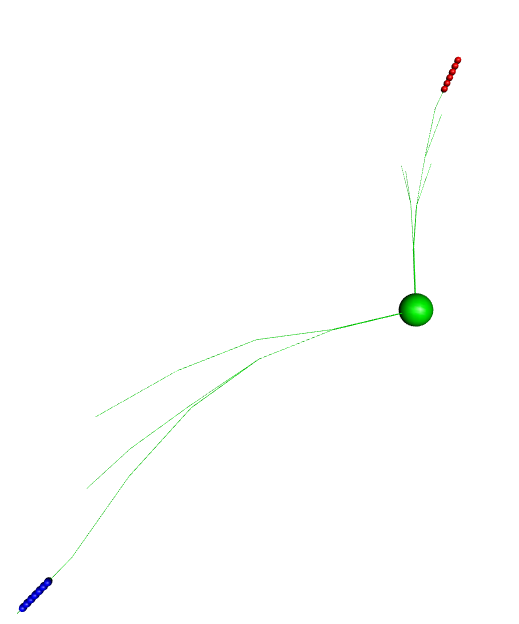
\includegraphics[width=\columnwidth]{./Images/pass_neuron.png} 
       % $BGX7J$OGr$NJ}$,NI$5$=$&(B
       % rgl$B$N;0<!852hA|$O(Beps$B$K$7$J$$$[$&$,$h$$(B
       \caption{$B?@7P:YK&$NNc(B}
       \label{Neuron}
     \end{subfigure}
     \begin{subfigure}{0.2\columnwidth}
       \centering
       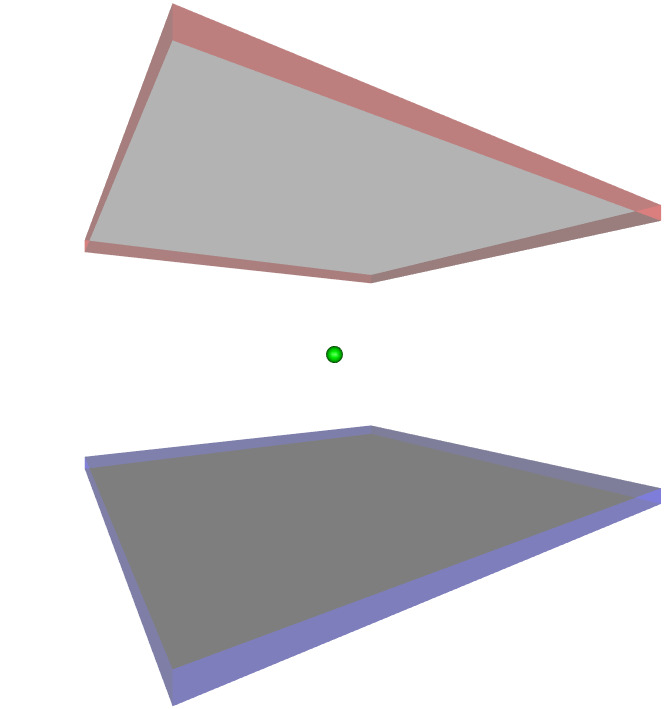
\includegraphics[width=\columnwidth]{./Images/synaptic_zone.png}
       \caption{$B%7%J%W%F%#%C%/%>!<%s(B}
       \label{synaptic-zone}
     \end{subfigure}
     \begin{subfigure}{0.4\columnwidth}
       \centering
       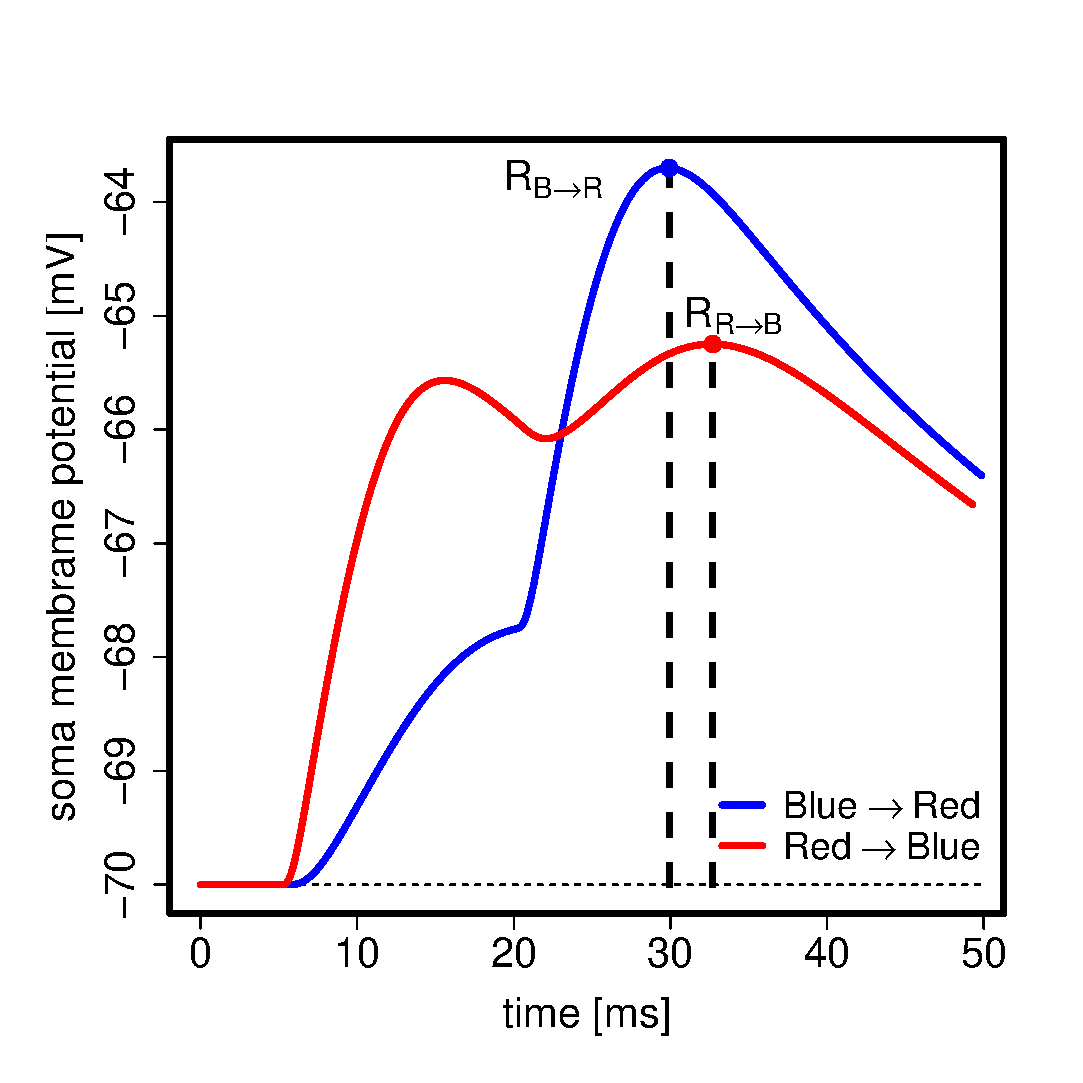
\includegraphics[width=\columnwidth]{./Images/input_order_detection.eps} 
       \caption{input-order detection}
       \label{input-order_detection}
     \end{subfigure}
     \caption{$B:n@.$7$??@7P:YK&$H(Binput-order detection}
     \label{sample}
   \end{figure}

 \section{$B?@7P:YK&7ABV$N:n@.J}K!(B}
   $B4JC1$N$?$a?@7P:YK&$N7ABV$O:YK&BN$H(B2$BK\$N<y>uFM5/$N$_$+$i$J$k$H$9$k(B.
   $B$^$?:YK&BN$N7ABV$O0lDj$NBg$-$5$N5e7A$G$"$k$H$9$k(B. 
   $B$h$C$F?@7P:YK&$N7ABV@8@.$O<y>uFM5/$N7ABV$r@8@.$9$k$3$H$G9T$o$l$k(B.
   $B<y>uFM5/7ABV$N@8@.$O3NN(E*$J<jK!$rMQ$$(B, $B7ABV$r:n@.$7$?8e$K%3%s%@%/%?%s%9$r(B
   $BJ,I[$5$;$k(B. 
   \subsection{$B?@7P:YK&7ABV$NI=8=(B}
     $B?@7P:YK&$N7ABV$r(B3$B<!856u4V>e$KI=8=$9$k(B. $B:YK&BN$OD>7B(B25$[{\rm{{\mu}m}}]$$B$N(B
     $B5e$H$7(B, $B<y>uFM5/$O1_Cl$N=89gBN$H$7$FI=8=$9$k(B. $B1_ClC<It$NCf?4ItJ,(B
     $B$OB>$N1_Cl$d:YK&BN$H7k9g$7(B, $B<y>u$N9=B$$r7A@.$9$k(B. $B$3$3$G(B, 1$BK\$N1_Cl$r(BBranch$B$HDj5A$9$k(B.
     $B$^$?:YK&BN$HD>@\7k9g$7$F$$$k(BBranch$B$rFC$K(BStem$B$H$9$k(B. 1$BK\$N(BStem$B$H(B, 
     $B$=$N(BStem$B$+$i?-$S$F$$$k(BBranch$B$+$i$J$k<y>u9=B$$r$"$o$;$F(B1$B$D$N<y>uFM5/(B(Dendrite)
     $B$G$"$k$HDj5A$9$k(B. $B$h$C$F(B1$B$D$N?@7P:YK&$O(BStem$B$NK\?t$@$1$N<y>uFM5/$r;}$D(B.
     $B$3$N?@7P:YK&7ABV$K4X$9$kDj5A$r0J2<$N?^(B\ref{morpho}$B$K<($9(B.
     \begin{figure}[H]
       \centering
       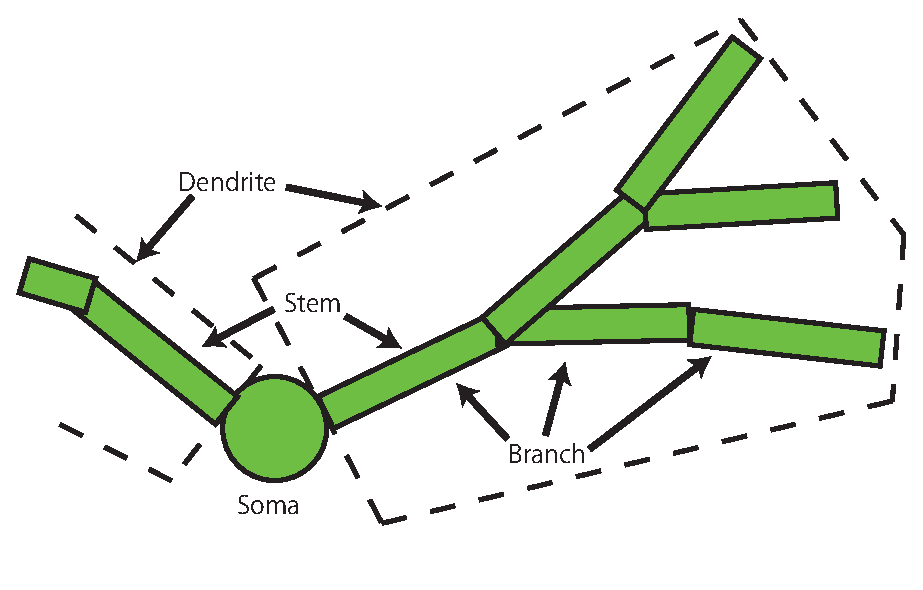
\includegraphics[width=10cm]{./Images/neuron_morpho.eps}
       \caption{$B?@7P:YK&7ABV$K4X$9$kDj5A(B}
       \label{morpho}
     \end{figure}
   \subsection{$B<y>uFM5/7ABV@8@.<jK!$N4pK\35G0(B}
     $B<y>uFM5/7ABV@8@.<jK!$N4pK\$O(BL-system$B$G$"$k(B.\cite{prusinkiewicz1990}
     L-system$B$O$"$k5-9f$N=89g$H$=$NCV$-49$(5,B'$+$iDj5A$5$l(B, $B=i4|>uBV$H$7$F$"$k5-9fNs$,M?$((B
     $B$i$l$k$H(B, $B$=$l$r:F5/E*$KJQ99$7$F$$$/%7%9%F%`$G$"$k(B. L-system$B$NNc(B
     \cite{torben2007evolving}$B$r<($9(B. $B$^$:5-9f$N=89g(B$\{B,F,X,Y\}$$BDj5A$9(B
     $B$k(B. $B<!$K$=$NCV$-49$(5,B'$H$7$F(B
     \begin{align*}
       rules: \hspace{0.2cm} & F \to YF\\
       & X \to BX
     \end{align*}
     $B$rDj5A$9$k(B. $B=i4|>uBV$H$7$F5-9fNs(B$FX$$B$,M?$($i$l$?$H$9$k$H(B,
     L-system$B$OCV$-49$(5,B'$K=>$C$F$3$N5-9fNs$NCV$-49$($r:F5/E*$K9T$&(B. 2$B2s(B
     $BL\$NCV$-49$(=*N;$^$G$N5-9fNs$NJQ2=$O0J2<$N$h$&$K$J$k(B.
     \begin{align*}
       initial:\hspace{0.2cm} & FX \\
       1^{st} cycle:\hspace{0.2cm} & YFBX \\
       2^{nd} cycel:\hspace{0.2cm} & YYFBBX
     \end{align*}
     $B<y>uFM5/7ABV$N@8@.J}K!$H$7$F(B, $B;05\(B et al$B$r;29M$K$9$k$H0J2<$N$h$&$J(BL-system$B$,9M$($i$l$k(B.\cite{$B;05\?.IW(B1998$B0dEA(B
       $B%"%k%4%j%:%`$H:GE,2=(B}
     $B;HMQ$9$k5-9f$N=89g$H$7$F(B$\{S,B,T\}$$B$rDj5A$9$k(B.$BCV$-49$(5,B'$H$7$F(B
     \begin{align*}
       rules: \hspace{0.2cm}
       & S \to
       \begin{cases}
         T & \text{(Termination)}\\
         \begin{cases}
           BS<BS> &\text{(Bifurcation)} \tag{$*$}\\
           BS &\text{(otherwise)}
         \end{cases} & \text{(otherwise)}
       \end{cases}\\
       & B \to B \\
       & T \to T
     \end{align*}
     $B$rDj5A$9$k(B. $B5-9f(B$S,B,T$$B$r<y>uFM5/$N9=B$$KCV$-49$($k$H(B, $B5-9f(BS$B$O<y>u(B
     $B9=B$$K$*$1$kL$@.D9$NE@$rI=$7(B, $B5-9f(BB$B$O(BBranch, $B5-9f(BT$B$O<y>uFM5/$NC<E@$KBP1~$9$k(B.
     $B$3$3$G(B, $<$\hspace{0.1cm}$>$$B$O<y>u9=B$$NJ,4t$rI=$7$F$$$k(B. $B$3$N(BL-System$B$O(B
     1$B$D$NL$@.D9E@$r=i4|>uBV$H$7(B, $B$=$3$+$i<y>u9=B$$,@8@.$5$l$F$$$/2aDx$rI=8=$9$k(B. 
     $B5-9f(BS$B$NCV$-49$(5,B'(B($*$)$B$O7hDjE*$G$O$J$/(B, $B8e$K=R$Y$kJ,4t3NN($d=*C<3NN($K$h$C$F7hDj(B
     $B$5$l$k(B. 1$B$D$N<y>uFM5/$O=i4|>uBV(B$\{S\}$$B$+$i(B, $B$3$N(BL-System$B$r3+;O$75-9fNs$,JQ(B
     $B2=$7$J$/$J$k$^$GCV$-49$($r9T$&$3$H$GF@$i$l$k(B. $B$^$?(B, $B:G$b:G=i$N5-9fCV$-49$($G$OI,$:(B$S \to BS$$B$N(B
     $BCV$-49$($,A*Br$5$l$k$h$&$K$9$k(B. \\
     $B:G=*E*$KF@$i$l$k5-9fNs$O5-9f(B$B$$B$H5-9f(B$T$$B$+$i$J$j(B, $B:G$b:8C<$K$"$k5-9f(B$B$$B$,(BStem$B$rI=$9(B. 

   \subsection{$B%Q%i%a!<%?%;%C%H(B, $Branch$, $Dendrite$, $Neuron$$B$NDj5A(B}
     1$B$D$N<y>uFM5/$O(B1$BAH$N%Q%i%a!<%?%;%C%H$+$i:n@.$5$l$k(B. $B$h$C$F(B1$B$D$N?@7P:YK&$O(B2$BAH$N(B
     $B%Q%i%a!<%?%;%C%H$r;}$A(B, $B$=$3$+$i(B2$BK\$N<y>uFM5/$,@8@.$5$l$k(B. 
     1$B$D$N%Q%i%a!<%?%;%C%H$K$O<y>uFM5/$N7ABV$r7hDj$9$k$?$a$N%Q%i%a!<%?$H<y>uFM5/>e$N(B
     $B%3%s%@%/%?%s%9J,I[$r7hDj$9$k$?$a$N%Q%i%a!<%?$,B8:_$9$k(B. $BA0<T$N%Q%i%a!<%?$r7ABV%Q%i%a!<%?(B, $B8e<T$N(B
     $B%Q%i%a!<%?$r%3%s%@%/%?%s%9%Q%i%a!<%?$H$9$k(B. 
     $BI=(B\ref{morpho_parameter}$B$O<y>uFM5/7ABV$r@8@.$9$k$?$a$K;HMQ$9$k%Q%i%a!<%?$G$"$k(B.

     \begin{table}[H]
       \caption{$B7ABV%Q%i%a!<%?(B}  % <- $B%Q%i%a!<%?$O:G8e$K$^$H$a$?J}$,$$$$$+$b(B
       \label{morpho_parameter}
       \begin{center}
         \begin{tabular}[H]{|l|l|c|} \hline
           \multicolumn{1}{|c}{$B%Q%i%a!<%?L>(B} & \multicolumn{1}{|c|}{$B@bL@(B} & \multicolumn{1}{c|}{$BCM0h(B}\\ \hline \hline
           1,  \textit{Segment Length} [${\rm {\mu}m}$]& Stem$B$*$h$S(BBranch$B$ND9$5(B & [$0,\infty$) \\ \hline
           2,  \textit{Stem diameter}  [${\rm {\mu}m}$]& Stem$B$ND>7B(B & [$0.15,\infty$) \\ \hline
           3,  \textit{Stem elevation} [$^{\circ}$]& Stem$B$N6D3Q(B & [$0,360$) \\ \hline
           4,  \textit{Stem rotation}  [$^{\circ}$]& Stem$B$N2sE>(B & [$0,360$) \\ \hline
           5,  \textit{Branch elevation $\mu$} [$^{\circ}$]& Branch$B$N6D3Q7hDj$KMQ$$$kJ?6QCM(B & [$0,360$) \\ \hline
           6,  \textit{Branch elevation $\sigma$} [$^{\circ}$] & Branch$B$N6D3Q7hDj$KMQ$$$kI8=`JP:9CM(B & [$0,\infty$) \\ \hline
           7,  \textit{Branch rotation $\mu$}  [$^{\circ}$]& Branch$B$N2sE>3Q7hDj$KMQ$$$kJ?6QCM(B & [$0,360$) \\ \hline
           8,  \textit{Branch rotation $\sigma$} [$^{\circ}$] & Branch$B$N2sE>3Q7hDj$KMQ$$$kI8=`JP:9CM(B & [$0,\infty$)  \\ \hline
           9,  \textit{Bifurcation} $\alpha$ & $B<y>u9=B$$NJ,4tF3F~H=Dj$KMQ$$$k(B$k$$BCM(B & [$1,\infty$) \\ \hline
           10, \textit{Bifurcation} $\beta$  & $B<y>u9=B$$NJ,4tF3F~H=Dj$KMQ$$$k(B$\theta$$BCM(B & [$1,\infty$) \\ \hline
           11, \textit{Termination} $\alpha$ & $B<y>u9=B$$N=*C<E@F3F~H=Dj$KMQ$$$k(B$k$$BCM(B & [$1,\infty$) \\ \hline
           12, \textit{Termination} $\beta$  & $B<y>u9=B$$N=*C<E@F3F~H=Dj$KMQ$$$k(B$\theta$$BCM(B & [$1,\infty$) \\ \hline
         \end{tabular}
       \end{center}
     \end{table}

     $B0J2<$K%3%s%@%/%?%s%9%Q%i%a!<%?$r<($9(B. $BK\8&5f$G$O<y>uFM5/>e$N%3%s%@%/%?%s%9J,I[$r7hDj$9$k:]$K(B
     $B@~7AJ,I[(B, $B$^$?$O%,%&%9J,I[$N$I$A$i$+$rMQ$$$k(B. $B<y>uFM5/>e$N%3%s%@%/%?%s%9$r@~7A$KJ,I[$5$;$k>l9g$OI=(B\ref{liner_parameter}$B$K<($5$l$k(B
     $B%Q%i%a!<%?$r(B, $B%,%&%9J,I[$K=>$C$FJ,I[$5$;$k>l9g$K$OI=(B\ref{gausian_parameter}$B$K<($5$l$k%Q%i%a!<%?$r$=$l$>$lMQ$$$k(B.

     \begin{table}[H]
       \caption{$B@~7AJ,I[%3%s%@%/%?%s%9%Q%i%a!<%?(B}
       \label{liner_parameter}
       \begin{center}
         \begin{tabular}[H]{|l|l|c|} \hline
           \multicolumn{1}{|c}{$B%Q%i%a!<%?L>(B} & \multicolumn{1}{|c|}{$B@bL@(B} & \multicolumn{1}{c|}{$BCM0h(B}\\ \hline \hline
           13, Ka \textit{Stem conductance} [${\rm S/cm^2}$]& Stem$B$N(BKa$B%3%s%@%/%?%s%9CM(B & [$0,0.22$] \\ \hline
           14, Ka \textit{taper rate}  & Ka$B%3%s%@%/%?%s%9$NEAHBN((B & [$0,\infty$) \\ \hline
           15, CaT \textit{Stem conductance} [${\rm S/cm^2}$]& Stem$B$N(BCaT$B%3%s%@%/%?%s%9CM(B & [$0,0.0022$] \\ \hline
           16, CaT \textit{taper rate}  & CaT$B%3%s%@%/%?%s%9$NEAHBN((B & [$0,\infty$) \\ \hline
         \end{tabular}
       \end{center}
     \end{table}

     \begin{table}[H]
       \caption{$B%,%&%9J,I[%3%s%@%/%?%s%9%Q%i%a!<%?(B}
       \label{gausian_parameter}
       \begin{center}
         \hspace*{-4em}
         \begin{tabular}[H]{|l|l|c|} \hline
           \multicolumn{1}{|c}{$B%Q%i%a!<%?L>(B} & \multicolumn{1}{|c|}{$B@bL@(B} & \multicolumn{1}{c|}{$BCM0h(B}\\ \hline \hline
           13, Ka \textit{peak} [${\rm S/cm^2}$]&  Ka$B%3%s%@%/%?%s%9J,I[$N:GBgCM(B & [$0,0.22$] \\ \hline
           14, Ka \textit{Gausian} $\mu$ & Ka$B%3%s%@%/%?%s%9J,I[$,=>$&%,%&%9J,I[$NJ?6QCM(B & [$0,1$] \\ \hline
           15, Ka \textit{Gausian} $\sigma$ & Ka$B%3%s%@%/%?%s%9J,I[$,=>$&%,%&%9J,I[$NI8=`JP:9CM(B & [$0,\infty$) \\ \hline
           16, CaT \textit{peak} [${\rm S/cm^2}$]&  CaT$B%3%s%@%/%?%s%9J,I[$N:GBgCM(B & [$0,0.0022$] \\ \hline
           17, CaT \textit{Gausian} $\mu$ & CaT$B%3%s%@%/%?%s%9J,I[$,=>$&%,%&%9J,I[$NJ?6QCM(B & [$0,1$] \\ \hline
           18, CaT \textit{Gausian} $\sigma$& CaT$B%3%s%@%/%?%s%9J,I[$,=>$&%,%&%9J,I[$NI8=`JP:9CM(B & [$0,\infty$) \\ \hline
         \end{tabular}
       \end{center}
     \end{table}

   $B$h$C$F(B1$BAH$N%Q%i%a!<%?%;%C%H$O7ABV%Q%i%a!<%?$K%3%s%@%/%?%s%9%Q%i%a!<%?$r2C$($?(B16, $B$^$?$O(B18$B9`L\$G9=@.$5$l$F$$$k(B. \\
   $B$R$H$D$N(BBranch$B$OD9$5(B($length$), $BB@$5(B($diam$), $B6D3Q(B($elevation$), $B2sE>3Q(B($rotation$)$B$r(B
   $B%Q%i%a!<%?$H$7$F;}$D(B. $B$h$C$F(B, $B$"$k(B$Branch_i$$B$O(B4$B$D$N%Q%i%a!<%?$+$i$J$j(B, 
   \begin{equation*}
    Branch_i = \{length_i, diam_i, elevation_i, rotation_i\}
   \end{equation*}
   $B$HI=$9$3$H$,$G$-$k(B. $B$^$?%$%s%G%C%/%9(B$i = 1$$B$N$H$-(B, $B$9$J$o$A(B$Branch_1$$B$O(BStem$B$G$"$k(B.
   $B$^$?(B$Dendrite$$B$O(B$Branch$$B$N=89g$G$"$j(B, 
   \begin{equation*}
     Dendrite_i = \{Branch_1,Branch_2,\dots,Branch_{N_i}\}
   \end{equation*}
   $B$^$?(B, 1$B$D$N?@7P:YK&(B($Neuron$)$B$O(B2$B$D$N(BDendrite$B$+$i$J$k(B. $B$h$C$F(B
   \begin{equation*}
     Neuron_i = \{Dendrite_1,Dendrite_2\}
   \end{equation*}
   $B$G$"$k(B. 

 \subsection{$Branch$$B7ABV%Q%i%a!<%?7hDjJ}K!(B}
   $B0J2<$K(B$Branch_i$$B$N%Q%i%a!<%?7hDjJ}K!$r=R$Y$k(B. $B$^$?(B, $B0J2<$N0lO"$N%Q%i%a!<%?7hDj<jK!$r(B
   $B4X?t(BmakeBranch($diam_{parent}$)$B$H$9$k(B. $B4X?t(BmakeBranch$B$O0z?t$H$7$F?F(BBranch$B$ND>7B(B$diam_{parent}$
   $B$r<h$j(B, $B?7$?$J(BBranch$B$rJV$94X?t$G$"$k(B. 
   \begin{enumerate}
    \item \textbf{$BD9$5(B({$length_i$})$B$N7hDj(B}\\
      $BD9$5(B$length_i$$B$O%Q%i%a!<%?%;%C%H$K$"$k(B
      \textit{Segment Length}$B$NCM$=$N$b$N$G$"$k(B. 
      \begin{equation}
        length_i = Segment\hspace{1mm} Length
      \end{equation}
    \item \textbf{$BB@$5(B($diam_i$)$B$N7hDj(B}\\
      Branch$B$,J,4t(B(Bifurcation $ 1 \to 21<21>$)$B$K$h$C$F@8@.$5$l$k$+?-D%(B(Elongation $1 \to 21$)$B$K$h$C$F@8@.$5$l$k$+(B
      $B$K$h$C$F7hDjJ}K!$,0[$J$k(B. 
      \begin{itemize}
        \item{$BJ,4t(B(Bifurcation)$B$N>l9g(B} \\
          $B?F$H$J$k(B$Branch$$B$NB@$5(B($diam_{parent}$)$B$rMQ$$$F(B, $B%,%&%9J,I[(B($\mu = diam_{parent},\sigma=0.05$)
          $B$K=>$&Mp?t$r@8@.$7(B, $B$=$NCM$r(B$diam_i$$B$H$9$k(B. 
          \begin{equation}
            diam_i = N(diam_{parent},(0.05)^2)
          \end{equation}
        \item{$B?-D%(B(Elongation)$B$N>l9g(B} \\
          Branch$B$,(BStem$B$G$"$k$+$I$&$+$K$h$C$F7hDjJ}K!$,0[$J$j(B, Stem$B$G$J$$>l9g$O?F$H$J$k(B$Branch$$B$NB@$5(B($diam_{parent}$)$B$r(B
          $B<B?tG\$7$?CM$rMQ$$$k(B
          \begin{equation}
            diam_i = 
            \begin{cases}
              Stem\hspace{1mm}diam & \text{(i = 1)}\\
              diam_{parent} \times taper\hspace{1mm}rate & \text{(otherwise)}\\
            \end{cases}\\
      \end{equation}
      $B$3$3$G(B, $taper\hspace{0.1cm}rate = 0.875$$B$G$"$j(B, $diam$$B$N8:?jN($rI=$9(B.
      \end{itemize}
    \item \textbf{$B6D3Q(B($elevation_i$)$B$N7hDj(B}\\
      {\textit diam}$B$HF1MM$K(BStem$B$G$"$k$+$I$&$+$G7hDjJ}K!$,0[$J$k(B. 
      \begin{equation}
        elevation_i = 
        \begin{cases}
          Stem\hspace{1mm}elevation & \text{(i = 1)}\\
          N(Branch\hspace{1mm}elevation\hspace{1mm}\mu,(Branch\hspace{1mm}elevation\hspace{1mm}\sigma)^2) & \text{(otherwise)}\\
       \end{cases}\\
      \end{equation}
    \item \textbf{$B2sE>3Q(B($rotation_i$)$B$N7hDj(B}\\
      $B6D3Q$N>l9g$HF1MM$K(B,
      \begin{equation}
        rotation_i = 
        \begin{cases}
          Stem\hspace{1mm}rotation & \text{(i = 1)}\\
          N(Branch\hspace{1mm}rotation\hspace{1mm}\mu,(Branch\hspace{1mm}rotation\hspace{1mm}\sigma)^2) & \text{(otherwise)}\\
       \end{cases}\\
      \end{equation}
   \end{enumerate}

 \subsection{$B5-9f(B1$B$NCV$-49$(5,B'(B($*$)}
   $B7ABV@8@.(BL-system$B$K$*$1$k5-9f(B$B$$B$O(BBranch$B$KBP1~$9$k(B.
   $B=i4|>uBV$N5-9f(B$S$$B$N:BI8$r86E@(B$(0,0,0)$$B$H$7(B, $B$"$k5-9f(B$S$$B$K;j(B
   $B$k$^$G$KDL2a$9$k(BStem$B$d(BBranch$B$N(B$length$$B$NOB$r(B${\rm path(S)}$$B$H$9$k(B. $B0J2<$K5-9f(B
   $S$$B$NCV$-49$(5,B'(B($*$)$B$NA*BrJ}K!$r<($9(B. 
   \begin{enumerate}
     \item \textbf{$BDd;_(B Termination $S \to T$} \\
        $[0,1]$$B$NHO0O$G0lMMJ,I[$K=>$&Mp?t$r0l$D@8@.$7(B, $B$=$NCM$r(B$rand$$B$H$9$k(B.
        $BN_@Q%,%s%^J,I[(B\textit{Cumulative} $\gamma$(x)$B$rMQ$$$F5-9f(B$S$$B$N?-D%Dd;_(B
        $B$NH=Dj$r9T$&(B. $B$=$N:](B, $BN_@Q%,%s%^J,I[$N%Q%i%a!<%?$H$7$F(B, $B%Q%i%a!<%?%;%C%H$N(B \\
        \begin{tabular}[c]{ll}
          - \textit{k} : & \textit{Termination} $\alpha$ \\
          - $\theta$ : &  \textit{Termination} $\beta$\\
        \end{tabular}\\
        $B$NCM$rMQ$$(B, 
        \begin{equation}
	  {\rm Cumulative}\hspace{0.1cm}\gamma\hspace{0.05cm}({\rm path(1_i)}) > rand
        \end{equation}
        $B$H$J$k>l9g(B, $ S \to T$$B$H$9$k(B.

      \item \textbf{$BJ,4t(B Bifurcation $ S \to BS<BS>$} \\
        Termination$B$r9T$o$J$+$C$?>l9g$N$_(BBifurcation$B$NH=CG$r9T$&(B. 
        $[0,1]$$B$NHO0O$G0lMMJ,I[$+$iMp?t$r0l$D@8@.$7(B, $B$=$NCM$r(B$rand$$B$H$9$k(B.
        $B:GBgCM$,(B0.8$B$K$J$k$h$&$K<B?tG\$7$?%,%s%^J,I[(B
        \textit{Scaled} $\gamma$(x)$B$rMQ$rMQ$$$FJ,4t$NH=Dj$r9T$&(B. 
        $B$?$@$7%,%s%^J,I[$N%Q%i%a!<%?$H$7$F(B, $B%Q%i%a!<%?%;%C%H$N(B\\
        \begin{tabular}[c]{ll}
          - \textit{k} : & \textit{Bifurcation} $\alpha$ \\
          - $\theta$ : &  \textit{Bifurcation} $\beta$\\
        \end{tabular}\\
        $B$rMQ$$(B, 
        \begin{equation}
	  Scaled\hspace{0.1cm}\gamma\hspace{0.05cm}(path(S)) > rand
        \end{equation}
        $B$N$H$-(B$ S \to BS<BS>$$B$H$9$k(B. $B$9$J$o$A(BmakeBranch($diam_i$)$B$h$j(B, $B?7$?$J(B$Branch$$B$r(B2$B$D@8@.$9$k(B. 
      \item \textbf{$B?-D%(B Elongation $S \to BS$} \\
        $B>e5-$N>r7o$rK~$?$5$J$+$C$?>l9g(B, $S \to BS$$B$H$9$k(B. 
        $B$9$J$o$A(BmakeBranch($diam_i$)$B$h$j(B, $B?7$?$J(B$Branch$$B$r(B1$B$D@8@.$9$k(B. 
    \end{enumerate}

   \subsubsection{$B7ABVE*%R%e!<%j%9%F%#%C%/(B}
    $B0J2<$N>r7o$K3:Ev$9$k>l9g$O6/@)E*$K?-D%Dd;_(B(Termination)$B$H$9$k(B. $B$3$l$O<y(B
    $B>uFM5/$H$7$FBEEv$J7ABV$rF@$k$?$a$KF3F~$9$k%R%e!<%j%9%F%#%C%/%9$G$"$k(B.    % <- $BBEEv$H$O(B?
    \begin{itemize}
      \item ${\rm path}(S) > 2000$$B$N$H$-(B
      \item $diam_{i} \le Minimum\hspace{1mm}diameter$ $B$N$H$-(B\\ % <- $B%Q%i%a!<%?$r$"$H$G$^$H$a$?$[$&$,$$$$$+!)(B
       $B$^$?(B, $B$3$N>l9g(B$Branch_{i}$$B$N(B$diam_{i}$$B$r(B$Minimum\hspace{1mm}diameter$$B$K@_Dj$7D>$9(B. 
    \end{itemize}

    \subsection{$Branch$$B$KBP$9$k;0<!85:BI8$N@_Dj(B}
     $length_i$, $elevation_i$, $rotation_i$$B$N>pJs$rMQ$$$F;0<!856u4V>e$G$N(B$Branch_i$$B$N:BI8>pJs$r(B
     $B@_Dj$9$k(B. $Branch$$B$N?-D%J}8~$O?F$H$J$k(BStem, Branch$B$N8~$-$K$"$o$;$?Aj(B
     $BBPE*$J:BI8<4$rMQ$$$F9M$($k(B. $B6qBNE*$K$O0J2<$N$h$&$K$9$k(B. 
     \begin{itemize}
     \item \textbf{Stem$B$N3QEY@_Dj(B}
       \begin{enumerate}
       \item $B6D3Q(B \\
	 $B6D3Q$r(B$elevation^{\circ}$$B$H$9$k(B. $B=i4|>uBV$H$7$F(BStem$B$O(B3$B<!856u4V(B
	 $B$N86E@$+$i(Bx$B<4$HF1$8J}8~$K?-$S$F$$$k$H$9$k(B. $B$3$N>uBV$+$i(BStem$B$r(Bz$B<4(B
	 $B$rCf?4$H$7$F1&$M$8$NJ}8~$K(B$elevation^{\circ}$$B2sE>$5$;$k(B.
	 $B$3$N:](By$B<4(B, x$B<4$bF1MM$K2sE>$r9T$$(B, $B$=$l$>$l(By'$B<4(B, z'$B<4$H(B
	 $B$9$k(B.
       \item $B2sE>3Q(B \\
	 $B<!$K(B, $B2sE>3Q$r(B$rotation^{\circ}$$B$H$9$k(B. $B6D3Q$HF1MM$K(B,
	 Stem$B$r(By'$B<4$N1&$M$8$N8~$-$K(B$rotation^{\circ}$$B2sE>$5$;$k(B. $B$^$?(B
	 x'$B<4(B, z$B<4$K$D$$$F$bF1MM$N2sE>$r9T$$(B, $B$=$l$>$l(Bx''$B<4(B, z'
	 $B<4$H$9$k(B.
       \end{enumerate}
     \item \textbf{Branch$B$N3QEY@_Dj(B} \\
       Stem$B$HF1MM$K9T$&(B. $B$?$@$7(B, $B$=$N(BBranch$B$N?F$H$J$k(BStem, Branch$B$K$h$C(B
       $B$F2sE>$rM?$($?(Bx'',y',z'$B<4$rMQ$$$k(B. 
     \end{itemize}
     $B:G=*E*$KF@$i$l$?<y>uFM5/7ABV$O:YK&BN$NI=LL$K@\$9$k$h$&$K(B, Stem$B$NJ}8~(B
     $B$KJ?9T0\F0$5$;$k(B. \\   

    \subsection{$B%7%J%W%F%#%C%/%>!<%s$H(B, $B<y>uFM5/$X$N%7%J%W%9$NIUM?(B}
     3$B<!856u4V>e$N86E@$K:YK&BN$rG[CV$7(B, $y$$B<4J}8~$N(B$170 < y < 190$$B$NHO0O$r(B % <- $B$3$NJU$N:BI8>pJs$rJQ?t$K$7$?$[$&$,$$$$$+$b(B
     Red$B%7%J%W%F%#%C%/%>!<%s(B, $y$$B<4J}8~$N(B$-170 > y > -190$$B$NHO0O$r(BBlue$B%7%J%W%F%#%C%/(B
     $B%>!<%s$HDj5A$9$k(B($B?^(B\ref{synaptic-zone}). $B%7%J%W%F%#%C%/%>!<%sFb$K(B$Branch$$B$,7A@.$5$l$?(B
     $B>l9g(B, $Branch$$B>e$K%7%J%W%9$rIUM?$9$k(B. % <- $B>\$7$/$+$1$?$i=q$-$?$$(B
      
  \section{$B?tM}%b%G%k(B}
     L-system$B$K$h$C$F:n@.$5$l$??@7P:YK&$O%^%k%A%3%s%Q!<%H%b%G%k$K$h$C$F(B
     $B$=$NKlEE0L$N5sF0$r%7%_%e%l!<%7%g%s$9$k(B. 
     $BC10l%3%s%Q!<%H%a%s%H$NKlEE0L(B($V_i$)$B$O0J2<$N<0$K$h$C$F7W;;$5$l$k(B.
     %g_leak$B$OJ?9UEE0L(B = -70$B$K$J$k$h$&$KD4@a$7$F$$$k(B
     \begin{equation}
       cm\frac{dV_i}{dt} = g_{leak}(V_i - E_{leak}) + I_{CaT} + I_{Ka}
       %$B$3$N(Bcm$B$O>.J8;z$+BgJ8;z$+(B?
       \label{V_i}
     \end{equation}
     $B%3%s%Q!<%H%a%s%H$NKl>e$K%7%J%W%9$,J,I[$7$F$$$k>l9g$O>e<0(B\ref{V_i}$B$N1&(B
     $BJU$K0J2<$N9`$rDI2C$9$k(B.
     \begin{equation}
       (e^{-\frac{t}{{\tau}2}} - e^{-\frac{t}{{\tau}1}})g_{syn}(V_i
       - E_{syn})
       \label{eq_syn}
     \end{equation}

     $B$^$?(B, $B%3%s%Q!<%H%a%s%H$KB>$N%3%s%Q!<%H%a%s%H$,7k9g$7$F$$$k>l9g$O0J2<$N<0(B\ref{next_comp}$B$r<0(B\ref{V_i}$B$KDI2C$9$k(B. 
     $i$$BHVL\$N%3%s%Q!<%H%a%s%H$K(B$j$$BHVL\$N%3%s%Q!<%H%a%s%H$,7k9g$7$F$$$k$H$9$k$H(B, 
     \begin{equation}
       g_{i,j}(V_j - V_i)
       \label{next_comp}
     \end{equation}

     $B$^$?(B, $B<0(B\ref{V_i}$B$N(B$I_{CaT}$, $I_{Ka}$$B$O(BMigliore et al$B$K<($5$l$k%$%*%s%A%c%M%k$N(B
     $B%b%G%k$rMxMQ$7$F$$$k(B.\cite{migliore1995computer}
     \begin{itemize}
       \item $BEE0L0MB87?(BT$B7?(B${\rm Ca^{2+}}$$BEEN.(B
         \begin{align}
           I_{CaT} &= g_{CaT} {\cdot} ghk(V,cai,cao) \\                   
           g_{CaT} &= \overline{g}_{CaT} {\cdot} m^2 {\cdot} h  \\
           KTF &= \left(\frac{25.0}{293.15}\right) {\cdot} (T + 273.15) \\
           f &= \frac{KTF}{2} \\
           nu &= \frac{V}{f} \\
           ghk &= -f {\cdot} \left(1.0 - \frac{C_i}{C_o} {\cdot} \exp(nu) \right) {\cdot} efun(nu) \\
           efun(z) &=
           \begin{cases}
             1 - \frac{z}{2} & |z| < 10^{-4} \\
             \frac{z}{(e^z - 1)} & otherwise \\
           \end{cases}
         \end{align}

         $B$^$?(B, CaT$B%3%s%@%/%?%s%9$N%2!<%HJQ?t(B($m$$B$*$h$S(B$h$)$B$N5sF0$O0J2<$NHyJ,J}Dx<0$K$h$C$FI=8=$5$l$k(B.
         
         \begin{align}
           {\tau}_{m}(V)\frac{dm}{dt} &= \frac{{\alpha}_m(V)}{{\alpha}_m(V) + {\beta}_m(V)} - m \\
           {\tau}_m(V) &= \frac{1}{{\alpha}_m(V) + {\beta}_m(V)} \\
           {\alpha}_m(V) &= 0.2{\cdot}\frac{-V + 19.26}{\exp(\frac{-V + 19.26}{10}) - 1} \\
           {\beta}_m(V) &= 0.009{\cdot}\exp(-\frac{V}{22.03})
         \end{align}

         \begin{align}
           {\tau}_{h}(V)\frac{dh}{dt} &= \frac{{\alpha}_h(V)}{{\alpha}_h(V) + {\beta}_h(V)} - h\\
           {\tau}_{h}(V) &= \frac{1}{{\alpha}_h(V) + {\beta}_h(V)} \\
           {\alpha}_h(V) &= 10^{-6}{\cdot}\exp(-\frac{V}{16.26}) \\
           {\beta}_h(V) &= \frac{1}{\exp(\frac{-V + 29.79}{10}) + 1}
         \end{align}

       \item A$B7?(BK$^+$$BEEN.(B
         \begin{align}
           I_{Ka} &= g_{Ka}{\cdot}(V - E_{K}) \\
           g_{Ka} &= \overline{g}_{Ka}{\cdot}n{\cdot}l
         \end{align}
         $B$^$?(B, Ka$B%3%s%@%/%?%s%9$N%2!<%HJQ?t(B($n$$B$*$h$S(B$l$)$B$N5sF0$O0J2<$NHyJ,J}Dx<0$K$h$C$FI=8=$5$l$k(B.
         \begin{align}
           {\tau}_n(V)\frac{dn}{dt} &= \frac{1}{1 + {\alpha}_n(V)} - n \\
           {\tau}_n(V) &= \frac{{\beta}_n(V)}{Q_{10}{\cdot}{\alpha}_{0n}{\cdot}(1 + {\alpha}_n(V))} \\
           {\alpha}_n(V) &= {\exp}\left(\frac{10^{-3}{\cdot}{\zeta}_n{\cdot}(V - V_{n\frac{1}{2}}){\cdot}9.648{\cdot}10^4}
                                             {8.315{\cdot}(273.16 + T)} \right) \\
           {\beta}_n(V) &= {\exp}\left(\frac{10^{-3}{\cdot}{\zeta}_n{\cdot}gm_n{\cdot}(V - V_{n\frac{1}{2}}){\cdot}9.648{\cdot}10^4}
                                             {8.315{\cdot}(273.16 + T)} \right)
         \end{align}

         \begin{align}
           {\tau}_l(V)\frac{dl}{dt} &= \frac{1}{1 + {\alpha}_l(V)} - l \\
           {\tau}_l(V) &= \frac{{\beta}_l(V)}{Q_{10}{\cdot}{\alpha}_{0l}{\cdot}(1 + {\alpha}_l(V))} \\
           {\alpha}_l(V) &= {\exp}\left(\frac{10^{-3}{\cdot}{\zeta}_l{\cdot}(V - V_{l\frac{1}{2}}){\cdot}9.648{\cdot}10^4}
                                             {8.315{\cdot}(273.16 + T)} \right) \\
           {\beta}_l(V) &= {\exp}\left(\frac{10^{-3}{\cdot}{\zeta}_l{\cdot}gm_l{\cdot}(V - V_{l\frac{1}{2}}){\cdot}9.648{\cdot}10^4}
                                             {8.315{\cdot}(273.16 + T)} \right)
         \end{align}
     \end{itemize}

     $B$?$@$7(B
     \begin{align}
       Q_{10} &= 3^{(\frac{T - 30}{10})}
     \end{align}
     $B$G$"$k(B.
%
% gmn gml$B$O2?$J$N$+!)(B g_{mn}$B$J$N$+!)(B $BC10L$OL5$$$h$&$J$N$G!"(Bgmn$B$@$H;W$&(B
%
     $B$^$?(B, $B%7%_%e%l!<%7%g%s$K4X$o$k%Q%i%a!<%?$r0J2<$NI=(B\ref{sim_para}$B$K<($9(B.

     \begin{table}[H]
       \caption{$B%7%_%e%l!<%7%g%s%Q%i%a!<%?(B}
       \label{sim_para}
       \begin{center}
	\begin{tabular}[t]{|c|c|} \hline
          \multicolumn{1}{|c}{$B%Q%i%a!<%?L>(B} & \multicolumn{1}{|c|}{$BCM(B} \\ \hline \hline
	 Simulation time [ms]& 50 $B$^$?$O(B 100 \\\hline % <- $B$3$3JQ$($k(B 2$BCJAH$_$NI=$K$9$k(B
	 $Ra$  [${\rm{\Omega}cm}$] & 100 \\ \hline
	 $Cm$  [${\rm{\mu}F/cm^2}$] & 0.8 \\ \hline
	 ${\tau}_{1}$ [ms] & 0.5\\ \hline
	 ${\tau}_{2}$ [ms] & 2\\ \hline
	 $V_{init}$ [mV]& -70\\ \hline
	 $g_{pas}$ [${\rm S/cm^2}$]& $2.5 \times 10^{-5}$\\ \hline
	 $E_{pas}$ [mV] & -70\\ \hline
	 $E_{K}$ [mV] & -91\\ \hline
	 $T$ [${\rm ^{\circ}C}$] & 37\\ \hline
         $\overline{g}_{CaT}$ [${\rm S/cm^2}$]& 0.003\\ \hline
         $\overline{g}_{Ka}$ [${\rm S/cm^2}$]& 0.01\\ \hline
         ${\alpha}_{0n}$ [${\rm ms^{-1}}$]& 0.02\\ \hline
         ${\alpha}_{0l}$ [${\rm ms^{-1}}$]& 0.08\\ \hline
         ${\zeta}_n$ & -3\\ \hline
         ${\zeta}_l$ & 4\\ \hline
         $gm_n$ & 0.6\\ \hline
         $gm_l$ & 1\\ \hline
         $V_{n\frac{1}{2}}$ [mV]& -33.6\\ \hline
         $V_{l\frac{1}{2}}$ [mV]& -83\\ \hline
         $C_i$ [mM]& $50{\times}10^{-6}$\\ \hline
         $C_o$ [mM]& 2\\ \hline
	\end{tabular}
       \end{center}
      \end{table}

 \section{$B:n@.$7$??@7P:YK&$N?tM}%b%G%k2=(B}
   L-System$B$K$h$C$FF@$i$l$??@7P:YK&$rA0@a$G<($7$??tM}%b%G%k$KJQ49$9$k<jK!$r<($9(B. 
   $B$R$H$D$N(B$Branch$$B$O:GBg(B5[$mu$m]$B$NBg$-$5$KJ,3d$7$F$=$l$>$l$K<0(B\ref{V_i}$B$rMQ$$$F(B
   $BKlEE0L$r7W;;$9$k(B. $B$"$k<B?t(B$x$$B$KBP$7$F(B, $x$$B0J>e$N:G>.$N@0?t$rJV$94X?t$r(Bceiling($x$)
   $B$H$9$k(B. $B$3$N$H$-(B, $B$"$k(B$Branch_i$$B$rJ,3d$9$k8D?t(B$d_i$$B$O(B, $Branch_i$$B$ND9$5(B$length_i$
   $B$rMQ$$$F0J2<$N$h$&$KDj5A$9$k(B. 
   \begin{align}
     d_i &= 
     \begin{cases}
       {\rm ceiling}(\frac{length_i}{5}) & \text{(${\rm ceiling}(\frac{length_i}{5})$ is odd)}\\
       {\rm ceiling}(\frac{length_i}{5}) + 1 & \text{(${\rm ceiling}(\frac{length_i}{5})$ is even)}\\
     \end{cases}\\
   \end{align}
   $B$3$3$G(B$d_i$$B$r4q?t$H$9$k$N$O%7%_%e%l!<%7%g%s$K(BNEURON$B$rMQ$$$F$$$k$?$a$G$"$k(B.\\ % <- $B$G$-$?$iM}M3$r=q$-$?$$(B
   $B$h$C$F(B, 1$B$D$N(B$Branch_i$$B$O(B$\frac{length_i}{d_i}$$B$ND9$5$4$H$K(B1$B$D$N%3%s%Q!<%H%a%s%H$KJ,3d$5$l(B$\{Comp_{i,j}\}$$B$H$J$k(B. 
   $\{Comp_{i,j}\}$$B$N$=$l$>$l$N%3%s%Q!<%H%a%s%H$K$D$$$F<0(B\ref{V_i}$B$rMQ$$$FKlEE0L$r7W;;$9$k(B. 

   %
   %
   % $B$3$N$X$s$G?^$r$$$l$k$H$o$+$j$d$9$$$+$b$7$l$J$$(B
   %

   \subsection{$B%3%s%Q!<%H%a%s%H>e$N%3%s%@%/%?%s%9J,I[@_Dj(B}
     $B:n@.$7$?%3%s%Q!<%H%a%s%H$N$=$l$>$l$K%3%s%@%/%?%s%9$r@_Dj$9$k(B. 
     $B%3%s%@%/%?%s%9J,I[$O@~7A$JJ,I[$H%,%&%9J,I[$N(B2$B$D$r2>Dj$7$?(B. $B@~7A$J%3%s%@%/%?%s%9J,I[$O@h9T8&5f$GMQ$$$i$l$F$$$?(B
     $B<jK!$G$"$k(B\cite{torben2009systematic}. $B%,%&%9J,I[$rMQ$$$k$N$O(B, $B@~7AJ,I[$N>l9g$h$j$b:Y$+$/%3%s%@%/%?%s%9J,I[$NJQ2=(B
     $B$rI=8=$7(B, $B$h$jB?$/$N%3%s%@%/%?%s%9J,I[%Q%?!<%s$rI=8=$9$k$?$a$G$"$k(B. 
     $B0J2<$K(B$Comp_{i,j}$$B$KBP$9$k%3%s%@%/%?%s%9CM$N7hDjJ}K!$r=R$Y$k(B. 
     $B%3%s%@%/%?%s%9CM$N7hDjJ}K!$O@~7AJ,I[$rMQ$$$k$+%,%&%9J,I[$rMQ$$$k$+$K$h$C$F0[$J$k(B. \\
     \begin{itemize}
     \item \textbf{$B@~7AJ,I[$N>l9g(B}\\
       $Branch$$BC10L$G%3%s%@%/%?%s%9$r@_Dj$9$k(B. $B$D$^$j$"$k(B$Branch_i$$B$+$iJ,3d$5$l$?%3%s%Q!<%H%a%s%H(B$\{Comp_{i,j}\}$$B$O(B
       $BA4$FF1$8%3%s%@%/%?%s%9CM$r;}$D(B. $Branch_i$$B$N%3%s%Q!<%H%a%s%H$N%3%s%@%/%?%s%9CM$r(B${g_{\rm CaT}}_{i,j}$, ${g_{\rm Ka}}_{i,j}$$B$H$7(B,
       $B>e5-$N(B$diam$$B$HF1MM$NJ}K!$G7hDj$9$k(B\\
       \begin{align}
         {g_{\rm CaT}}_{i,j} &= 
         \begin{cases}
           {\rm CaT}\hspace{1mm}Stem\hspace{1mm}conductance & \text{(i = 1)}\\
           {g_{\rm CaT}}_{{parent_i},j} \times {\rm CaT}\hspace{1mm}taper\hspace{1mm}rate & \text{(otherwise)}\\
         \end{cases} \\
                     {g_{\rm Ka}}_{i,j} &= 
                     \begin{cases}
             {\rm Ka}\hspace{1mm}Stem\hspace{1mm}conductance & \text{(i = 1)}\\
             {g_{\rm Ka}}_{{parent_i},j} \times {\rm Ka}\hspace{1mm}taper\hspace{1mm}rate & \text{(otherwise)}\\
           \end{cases}\\
         \end{align}

       \item \textbf{$B%,%&%9J,I[$N>l9g(B}\\
         $B%3%s%Q!<%H%a%s%HC10L$G%3%s%@%/%?%s%9CM$r@_Dj$9$k(B. Stem$B$+$i(B$Comp_{i,j}$$B$^$G$N(B$length$$B$N9g7W$r(Bpath($Comp_{i,j}$)$B$H$7(B, 
         $B$^$?$=$N<y>uFM5/A4BN$N%3%s%Q!<%H%a%s%H$G$N:GBg$N(Bpath($Comp_{i,j}$)$B$r(Bmax(Path($Comp_{i,j}$))$B$H$9$k(B. $B$3$N$H$-J?6QCM(B$\mu$, 
         $BI8=`JP:9(B$\sigma$$B$N%,%&%9J,I[$+$i<B?t(B$x$$B$KBP$9$k3NN(L)EY$r7W;;$9$k4X?t(BG($x,\mu,{\sigma}^2$)$B$K$D$$$F(B
         \begin{align}
           {\rm CaT}\hspace{1mm}Gaus\hspace{1mm}Max &= {\rm G}({\rm CaT}\hspace{1mm}Gausian\hspace{1mm}\mu,{\rm CaT}\hspace{1mm}Gausian\hspace{1mm}\mu,({\rm CaT}\hspace{1mm}Gausian\hspace{1mm}\sigma)^2) \\
           {\rm Ka}\hspace{1mm}Gaus\hspace{1mm}Max &= {\rm G}({\rm Ka}\hspace{1mm}Gausian\hspace{1mm}\mu,{\rm Ka}\hspace{1mm}Gausian\hspace{1mm}\mu,({\rm Ka}\hspace{1mm}Gausian\hspace{1mm}\sigma)^2)
         \end{align}
         $B$H$7(B, 

       \begin{align}
         {g_{\rm CaT}}_{i,j} &= {\rm G}(\frac{{\rm path}(Comp_{i,j})}{{\rm max(Path}(Comp_{i,j}))},{\rm CaT}\hspace{1mm}Gausian\hspace{1mm}\mu,({\rm CaT}\hspace{1mm}Gausian\hspace{1mm}\sigma)^2) \\
         {g_{\rm Ka}}_{i,j} &= {\rm G}(\frac{{\rm path}(Comp_{i,j})}{{\rm max(Path}(Comp_{i,j}))},{\rm Ka}\hspace{1mm}Gausian\hspace{1mm}\mu,({\rm Ka}\hspace{1mm}Gausian\hspace{1mm}\sigma)^2) \\
       \end{align}


         %
         %
         %$B$3$3$b?^$rF~$l$?J}$,$$$$(B
         %


       \end{itemize}

   \subsection{$BC10l%3%s%Q!<%H%a%s%H$X$N%7%J%W%9$NIUM?(B}
     $B>e5-$N$h$&$KJ,3d$7$?%3%s%Q!<%H%a%s%H(B$i$$B$,0lItJ,$G$b(B$170 < y < 190$$B$NNN0h$KF~$C$F$$$?>l9g(B,  % <- $B$3$NJU$N:BI8>pJs$rJQ?t$K$7$?$[$&$,$$$$$+$b(B
     Red$B%7%J%W%9%0%k!<%W$KB0$9$k%7%J%W%9$rIUM?$9$k(B. $B6qBNE*$K$O%3%s%Q!<%H%a%s%H(B$i$$B$N(B
     $BKlEE0L$r<($9<0(B\ref{V_i}$B$N1&JU$K(B\ref{eq_syn}$B$r2C$($k(B. $B$^$?(B, y$B<4J}8~$N(B$-170 > y > -190$$B$KF~$C$F$$$?>l9g(B
     $B$O(BBlue$B%7%J%W%9%0%k!<%W$KB0$9$k%7%J%W%9$rIUM?$9$k(B. 

   \section{$B%7%_%e%l!<%7%g%s(B}
     $B:n@.$7$??@7P:YK&$N5!G=@-$rD4$Y$k$?$a(B, NEURON$B%7%_%e%l!<%?$rMQ$$$F(B
     $B?@7P:YK&KlEE0L$N5sF0$r%7%_%e%l!<%H$7$?(B. $B?@7P:YK&$N%7%J%W%9$r$"$k;~9o$K3h@-2=(B
     $B$5$;$k$3$H$GF~NOEEN.$rM?$((B, $B:YK&BN$K$*$1$k:GBgC&J,6KNL$r4Q;!$9$k(B. 
     Blue$B%7%J%W%F%#%C%/%>!<%s$KB0$9$k%7%J%W%9$r3h@-2=$5$;$k;~4V$r(B$t_{Blue}$, 
     Red$B%7%J%W%F%#%C%/%>!<%s$KB0$9$k%7%J%W%9$r3h@-2=$5$;$k;~4V$r(B$t_{Red}$, $B$H$9$k(B.
     $B:n@.$7$?(B1$B$D$N?@7P:YK&$KBP$7$F0J2<$NI=(B\ref{sim_protcol}$B$K<($9(B4$B$D$N%7%_%e%l!<%7%g%s$r9T$C$?(B. 
     $B$^$?(B, Blue$B%7%J%W%F%#%C%/%>!<%s(B, $B$^$?$O(BRed$B%7%J%W%F%#%C%/%>!<%s$KB0$9$k%7%J%W%9$,$J$$?@7P:YK&$K(B
     $B$D$$$F$O$3$N%7%_%e%l!<%7%g%s$r9T$o$J$+$C$?(B. 

     \begin{table}[H]
       \caption{$B%7%_%e%l!<%7%g%s%W%m%H%3%k(B}
       \label{sim_protcol}
       \begin{center}
	\begin{tabular}[t]{|l|c|c|} \hline
           & $t_{Blue}$ & $t_{Red} $ \\ \hline \hline
          1, Blue$B%7%J%W%F%#%C%/%>!<%sC1FH$G$NH/2P(B & 5 & - \\ \hline
          2, Red$B%7%J%W%F%#%C%/%>!<%sC1FH$G$NH/2P(B  & - & 5 \\ \hline
          3, Blue$B%7%J%W%F%#%C%/%>!<%s(B $\to$ Red$B%7%J%W%F%#%C%/%>!<%s$NH/2P(B & 5 & $5 + {\Delta}t$ \\ \hline
          4, Red$B%7%J%W%F%#%C%/%>!<%s(B $\to$ Blue$B%7%J%W%F%#%C%/%>!<%s$NH/2P(B & $5 + {\Delta}t$ & 5 \\ \hline
	\end{tabular}
       \end{center}
      \end{table}
     
     $B$3$3$G(B${\Delta}t[ms]$$B$OFs$D$N%7%J%W%972$+$i$NF~NO$N;~4V:9$G$"$j(B, $B0J2<$NI=(B\ref{Delta_t}$B$K<($9(B6$B$D$NCM$r$=$l$>$lMQ$$$?(B. 
     
     \begin{table}[H]
       \caption{${\Delta}t$}
       \label{Delta_t}
       \begin{center}
	\begin{tabular}[t]{|c|c|c|c|c|c|} \hline
          5 & 10 & 15 & 20 & 25 & 30 \\ \hline
	\end{tabular}
       \end{center}
      \end{table}


     $B%7%_%e%l!<%7%g%s$O(BNEURON$B%7%_%e%l!<%?$rMQ$$(B, CVode$B%"%k%4%j%:%`$rMQ$$$F9T$C$?(B. % <- NEURON $B%7%_%e%l!<%?$K4X$7$F=q$$$?J}$,$$$$$+!)(B
     CVode$B%"%k%4%j%:%`$rMQ$$$k:]$N%(%i!<$O(B$10^{-5}$$BL$K~$K@_Dj$7$?(B. 


 \section{$B0dEA%"%k%4%j%:%`(B}    % <- $B!V0dEA%"%k%4%j%:%`!W$H$$$&L>A0$O$I$&$J$N$+!)(B
   2$BAH$N%Q%i%a!<%?%;%C%H$r(B1$B$D$N8DBN$H$7$F(B200$B8DBN(B, $B@$Be?t(B500$B$G0dEA%"%k%4(B
   $B%j%:%`$rMQ$$$?%Q%i%a!<(B % <- $B0dEA%"%k%4%j%:%`$N%Q%i%a!<%?$b$I$3$+$GI=$K$^$H$a$?J}$,$$$$(B
   $B%?:GE,2=$r9T$C$?(B. 
   1$BAH$N%Q%i%a!<%?%;%C%H$r%Y%/%H%k(B$\overrightarrow{P}_i = \{p_{i,1},p_{i,2},\dots \}$
   $B$HI=$9$H(B, $B0l$D$N8DBN$O(B$u_i = \{\overrightarrow{P}_{i,1},\overrightarrow{P}_{i,2}\}$$B$HI=$5$l$k(B. 
   $B$^$?(B$\overrightarrow{P}_i$$B$+$i@8@.$5$l$k<y>uFM5/$r(B$Dend_i$$B$H$9$k(B. $B$h$C(B
   $B$F(B1$B$D$N8DBN(B$u_i$$B$+$i@8@.$5$l$k?@7P:YK&$O(B$Neuron_i = \{Dend_{i,1},Dend_{i,2}\}$$B$HI=$5$l$k(B.   
   $B$^$?(B, $B$"$k@$Be?t(B$g$$B$G$N(B$i$$BHVL\$N8DBN$r(B$u_{i,g}$$B$HI=$9$H$9$k(B.
   $B$3$N0dEA%"%k%4%j%:%`$K$*$1$k0dEA;R$O8DBN(B$u_{i,g}$$B$N;}$D%Q%i%a!<%?%;%C%H(B$P_{i,g,1},P_{i,g,2}$$B$G$"$k(B. 
   $BK\8&5f$N0dEA%"%k%4%j%:%`$G$O(B, $B%(%j!<%HJ]B8(B, $B0lE@8r:5(B, $BFMA3JQ0[$rMQ$$$?(B. $B0J2<$K$=$N>\:Y$r=R$Y$k(B. 
   \subsection{$B8DBNI>2A(B}
     $B>e=R$NDL$j3F?@7P:YK&$N7ABV$r@8@.$7%7%_%e%l!<%7%g%s$r9T$$(B, $B$=$N7k2L$r(B  % <- $B%7%_%e%l!<%7%g%s$H$$$&8@$$J}$ONI$/$J$$(B F$BCM%F%9%H$H$+6qBNE*$K(B
     $B$b$H$K8DBN$NI>2A$r9T$&(B. $B8DBN$NI>2A$K$O(B, $B8DBN$N5!G=@-(B\ref{F}$B$N$[$+8DBN(B
     $B$NBN@Q(B, $BJ,I[$9$k%3%s%@%/%?%s%9$NNL$r9MN8$9$k(B. 
     $B$7$+$7(B, $B8DBN$K$h$C$F$O>e2<$N%7%J%W%F%#%C%/%>!<%s$K<y>uFM5/$r?-$P$;$:(B, 
     $B$=$b$=$b%7%_%e%l!<%7%g%s$r9T$&$3$H$,$G$-$J$$$b$N$,H/@8$9$k$3$H$b$"$k(B.
     $B$^$??@7P:YK&$r$h$j<BJ*$K6a$E$1$k$3$H$H(B, $BBEEv$J%7%_%e%l!<%7%g%s$r9T$&$3$H$r(B % <- $BBEEv$H$O!)(B
     $BL\E*$H$7$F$$$/$D$+$N%R%e!<%j%9%F%#%C%/%9$rF3F~$7$?(B. 
     $B$^$?(B, $B@$Be?t(B$g$, $BE:$(;z(B$i$$B$N8DBN$NI>2ACM(B$E$$B$r(B$E_{i,g}$$B$HI=5-$9$k(B
     $B0J2<$K8DBN$NI>2AJ}K!$r=R$Y$k(B. \\
     \begin{itemize}
       \item \textbf{$B7ABVE*%(%i!<(B}\\
         $BN>J}$N%7%J%W%F%#%C%/%>!<%s$K%7%J%W%9$r;}$?$:%7%_%e%l!<%7%g%s$r9T$($J$$8DBN$N>l9g(B
         $Dend_{i,1}$$B$N(B$y$$B:BI8$N:GBgCM$r(Bmax($y_1$), $Dend_{i,2}$$B$N(B$y$$B:BI8$N:G>.CM$r(Bmin($y_2$)$B$H$7(B % <- $B$3$N$X$s$b=q$-D>$9(B
         $BI>2ACM(B$E_{i,g}$$B$r(B
         \begin{equation}
           E_{i,g} = -{\rm max}\left(170 - {\rm max}(y_1),0\right) + {\rm min}\left(-170 - {\rm min}(y_2),0\right) - 100
           \label{Morpho_E}
         \end{equation}
         $B$H$9$k(B. 

       \item $B%7%_%e%l!<%7%g%s$r9T$C$?8DBN$K4X$7$F$O0J2<$NI>2A<0$K$h$C$FI>2ACM(B$E_{i,g}$$B$rM?$($k(B. 
         \begin{align}
           Function Minus_{i,g} &= \frac{F_{i,g}}{F_{max,g}} \\
           Morphology Minus_{i,g} &= \frac{Volume_{i,g}}{Volume_{max,g}} \\
           Conductance Minus_{i,g} &= \frac{Conductance ratio_{i,g}}{Conductance_{max,g}} \\ %$B$"$H$G>\$7$/=q$/(B
         \end{align}

         \begin{equation}
           E_{i,g} = 100 - Function\hspace{1mm}Minus_{i,g} - Morphology\hspace{1mm}Minus_{i,g} - Conductance\hspace{1mm}Minus_{i,g}
         \end{equation}
     \end{itemize}

     $B$^$?(B, $B0J2<$N%R%e!<%j%9%F%#%C%/%9$K3:Ev$9$k8DBN$O(B, $B0J2<$N<0$K$h$C$FI>2A$9$k(B. %$B>e$N<0$H$N4XO"$O(B?
     \begin{itemize}
       \item \textbf{$B7ABVE*%R%e!<%j%9%F%#%C%/%9(B}\\
         $B0J2<$N>l9g$O%7%_%e%l!<%7%g%s$r9T$o$:(B, $B<0(B\ref{Morpho_E}$B$K$h$C$FI>2ACM(B$E_{i,g}$$B$rM?$($?(B. 
         \begin{itemize}
           \item $B?@7P:YK&A4BN$G(BStem$B$H(BBranch$B$N8D?t$,9g7W(B15$BL$K~$N>l9g(B
           \item $B?@7P:YK&A4BN$G<y>uFM5/$NJ,4t$,0l$D$b$J$$>l9g(B
         \end{itemize}
       \item \textbf{$B%7%_%e%l!<%7%g%s%R%e!<%j%9%F%#%C%/%9(B}\\
         $B0lJ}$N%7%J%W%F%#%C%/%>!<%s$N$_$G$NH/2P$K$h$k:YK&BN$G$NKlEE0L$NC&J,6K$,(B2mV$B0J2<$N>l9g0J2<$N>l9g$O(B % <- $B$o$+$j$K$/$$$N$G=q$-D>$9(B
         $\mu = -50$, $\sigma = 5$$B$N%,%&%9J,I[$+$iMp?t$r(B1$B$DH/@8$5$;(B, $B$=$NCM$rI>2ACM(B$E_{i,g}$$B$H$7$?(B.
         \begin{equation}
           E_{i,g} = N(-50,5^2) % <- $B$3$N=q$-J}$O$"$C$F$k$N$+(B
         \end{equation}

         $B$^$?(B, $B?@7P:YK&$NKl>u$K(BKa$B%A%c%M%k(B, CaT$B%A%c%M%k$rJ,I[$5$;$?>l9g$O0J2<$N>l9g$K$b>e<0$K$h$C$FI>2ACM$rM?$($k(B. 
         $B$3$l$O?@7P:YK&$G$NH/2P$d(B, $BKlEE0L$N?6F0$r(B % <- $B:YK&BN$G$NH/2P$rM^@)$9$k0UL#$O(B? $B$3$3%3%s%@%/%?%s%9$N;~$N$_$N9MN8$K$7$J$/$F$b$h$5$=$&(B
         $BM^@)$9$k$?$a$G$"$k(B.
         \begin{itemize}
           \item $B:YK&BN$G$NC&J,6KNL$,(B25mV$B$rD6$($?>l9g(B
	   \item $B%7%_%e%l!<%7%g%s$N:G8e$N(B5$B%9%F%C%W$GKlEE0L$N>e>:$,5/$3$C(B
	     $B$?>l9g(B
         \end{itemize}
     \end{itemize}

   $B$h$C$FI>2ACM$O(B100$B$K6a$$$[$INI$$I>2A$G$"$k(B. % <- $BI>2ACM$NJ,I[$K$D$$$F!"AX$K$J$k$3$H$r?^<($9$k$+!)(B

   
   \begin{figure}[h]
     \centering
     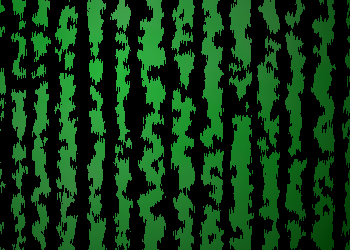
\includegraphics[width=5cm]{./Images/temp.png} 
     \caption{$BI>2ACM(B}
     \label{Estimate}
   \end{figure}

   \subsection{$B%(%j!<%HJ]B8(B}
      $B@$Be(B$g$$B$K$*$$$F:GBg$NI>2ACM$r$H$C$?8DBN$O(B, $B$=$N$^$^(B$g + 1$$B@$Be$N(B1$B8DBN$K0z$-7Q$,$l$k(B.
      $B@$Be(B$g$$B$K$*$$$F$N8DBN$NE:$(;z$rI>2ACM$NBg$-$5=g$KJB$Y(B, $B=g0L(B$k$$B$NE:$(;z$r(B$r_k$$B$GI=$9(B
      $B$H$9$k(B.$B$3$N$H$-%(%j!<%HJ]B8$O(B
      
      \begin{equation}
       u_{1,g + 1} = u_{r_1,g}
      \end{equation}
      
      $B$HI=8=$G$-$k(B.
   \subsection{$B0lE@8r:5(B, $BFMA3JQ0[(B}
   %$B8r:5!"FMA3JQ0[$r5/$3$98DBN$N?t$OCf?46K8BDjM}E*$J9M$($G5a$a$i$l$k(B
     $B<!@$Be$N%(%j!<%H0J30$N8DBN$O0lE@8r:5$^$?$OFMA3JQ0[$N$I$A$i$+$N<jK!$K$h$C$F:n@.$5$l(B
     $B$k(B. $B0lE@8r:5$OI>2ACM>e0L(B$\mu$$B8D$N8DBN(B($u_{r_{1},g},u_{r_{2},g},\dots,u_{r_{\mu},g}$)$B$r?F$H$7$F(B, $\lambda$$B8D$N;R8DBN(B % <- $B0dEAE*%"%k%4%j%:%`$K4X$9$k%Q%i%a!<%?$b8e$GI=$K$^$H$a$k(B
     $B$r@8@.$9$k(B. $B$3$N(B$\lambda$$B8D$N;R8DBN$OI>2ACM2<0L(B$\lambda$$B8D$N8DBN$H8r(B% <- $B$3$N&K$N7h$aJ}$,LdBj(B
     $B49$5$l$k(B. $BFMA3JQ0[$O;D$j$N(B$199 - \lambda$$B8D$N8DBN$KBP$7$FE,MQ$5$l$k(B.
     % <- $B$=$b$=$b$3$N(B($B&L(B,$B&K(B)$BK!$,$"$C$F$$$k$N$+$I$&$+!)(B
     $B$3$3$G(B$\mu = 10$$B$G$"$k(B. $B$3$3$G(B$Parents_g =
     \{u_{r_{1},g},u_{r_{2},g},\dots,u_{r_{\mu},g}\}$$B$H$7(B, Cross
     over($Parents$)$B$r0lE@8r:9$+$i<!@$Be8DBN$r0l$D:n@.$9$k4X?t$H$7(B,
     Mutation($u_{i.g}$)$B$r8DBN$KFMA3JQ0[$rM?$($k4X?t$G$"$k$H$9$k$H(B, $B<!@$(B
     $BBe8DBN(B$U_{g + 1}$$B$O(B
     \begin{equation}
      U_{g + 1} = \left(
       \begin{array}{c}
	u_{r_{1},g}, \\
	{\rm Cross\hspace{1mm}over(Parent_g)}_{2,g + 1}, \\
	\dots \\
	{\rm Cross\hspace{1mm}over(Parent_g)}_{1 + \lambda,g + 1}, \\ % <- $B$3$l$O$o$+$j$K$/$$(B
	{\rm Mutation(u_{r_{1},g})}, \\
	\dots \\
	{\rm Mutation(u_{r_{199 - \lambda},g})}
       \end{array}
       \right)
     \end{equation}
     
     \begin{itemize}
       \item \textbf{$B0lE@8r:5(B Cross over}\\
	     $BI>2ACM>e0L$N(B$\mu$$B8DBN$+$i3NN(E*$K?F$r(B2$B8DBNA*Br$9$k(B. $B?F$rA*Br$9(B
	     $B$k:]$K$O0J2<$N<0(B\ref{Parent_P}$B$KDj5A$9$k3NN(J,I[$rMQ$$$F(B,
	     $B?F$NE:$(;z$r;XDj$9$k(B. $BI>2ACM$,(B$k$$BHVL\$N(B % <- $BI>2ACM$,Ii$N8DBN$J$I$bB8:_$7!"%k!<%l%C%HA*Br$J$I$,;H$($J$$$H$$$&$3$H$b=q$/(B
	     $B8DBN$,A*Br$5$l$k2DG=@-$r(B$P_k$$B$H$7(B, 
	     \begin{equation} % $BA*Br3NN($r1_%0%i%U$G?^<($9$k$+!)(B
	      P_k =  
	       \begin{cases}
		(\frac{1}{2})^k &  k < \mu\\
		(\frac{1}{2})^{k - 1} & otherwise
		 \end{cases}\\
	      \label{Parent_P}
	     \end{equation}
	     $B$H$9$k(B.
	     $B$J$*(B, $BF1$88DBN$,=EJ#$7$FA*Br$5$l$J$$$h$&$K$7$?(B. \\
	     $BA*Br$5$l$?(B2$B$D$N?F8DBN$NE:$(;z$r(B$x$, $Py$$B$H$9$k(B. 
	     $B0lE@8r:5$O?F$N%Q%i%a!<%?%;%C%H(B$P_{i,g,1}$$BF1;N(B, $B%Q%i%a!<%?%;%C(B
	     $B%H(B$P_{i,g,2}$$BF1;N$G0J2<$N$h$&$K9T$&(B. %$B$J$<(BAB$B$rJ,$1$k$N$+$r=q$$$?J}$,$o$+$j$d$9$$(B
	     $B$3$l$O(B2$B$D$N(B$Dend_{i,1}$, $Dend_{i,2}$$B$r$=$l$>$lJL$N7OE}$H$7(B
	     $B$FE,1~$5$;$k$?$a$G$"$k(B.
         \begin{itemize}
           \item \textbf{$B8r:9E@$N7hDj(B} \\ %passive$B$N>l9g$O(BK,Ca$B%3%s%@%/%?%s%9$K4X$9$kItJ,$O8r:5$r9T$C$F$bL50UL#$@$C$?(B
             $B%Q%i%a!<%?%;%C%H$N9`L\?t$r(B$N_{Param}$$B$H$9$k(B. $B$3$N$H$-8r:9E@(B
		 \textit{Cross}$B$O(B$[N_{min},N_{max}]$$B$+$i(B
             $B0lMM$J3NN($G@0?t$r(B1$B$DJV$94X?t(BrandN($N_{min}$,$N_{max}$)$B$rMQ$$$F(B
             \begin{equation}
               Cross = {\rm randN}(1,N_{Param} - 1)
             \end{equation}
             $B$H$9$k(B. 
           \item \textbf{$B8r:5$N<B9T(B} \\
		 $B?7$?$J%Q%i%a!<%?%;%C%H$r:n@.$9$k(B. $B?7$?$J%Q%i%a!<%?%;%C%H$r(B
		 $\overrightarrow{P}_{new,i}$$B$H$9$k$H(B, $B?F$N%Q%i%a!<%?(B
		 $B%;%C%H(B$\overrightarrow{P_{x}}_{i}$,
		 $\overrightarrow{P_{y}}_{i}$$B$rMQ$$$F(B
		 \begin{equation}
		  \overrightarrow{P_{new}}_{i} = \{ p_{x,i,1}, p_{x,i,1}
		   \dots p_{x,i,Cross}, p_{y,i,Cross + 1},
		   p_{y,i,Cross + 2} \dots p_{y,i,N_{Param}}\} %$BE:$(;z$,Hs>o$KHQ;((B
		 \end{equation}
 
		 
         \end{itemize}
       \item \textbf{$BFMA3JQ0[(B Mutation}\\
        $B%Q%i%a!<%?%;%C%H$N3F9`L\$KBP$7$F(B0.65$B$N3NN($G%,%&%9J,I[(BG($\mu$,${\sigma}_M$)$B$K=>$&JQF0$rM?$($k(B. $B$9$J$o$A(B, $B$"$k%Q%i%a!<%?CM(B
         $p_i$$B$KBP$7$F(B, $B?7$7$$%Q%i%a!<%?CM(B${p'}_i$$B$O(B
         \begin{equation}
           {p'}_i = p_i + N(p_i,{{\sigma}_M}^2)
           \label{Mutation}
         \end{equation}
         $B$H$J$k(B. $B$3$3$GMQ$$$k(B${\sigma}_M$$B$O%Q%i%a!<%?$K$h$C$F0J2<$NI=(B\ref{sigma_M}$B$K<($5$l$k(B
         $BCM$rMQ$$$k(B. $B$3$l$O%Q%i%a!<%?$K$h$C$FCM$N%l%s%8$,0[$J$k$?$a$G$"$k(B. % <- $B%l%s%8!)(B
         ${p'}_i$$B$,I=(B\ref{sigma_M}$B$K<($5$l$kCM0h$K<}$^$i$J$$>l9g$O:FEY(B\ref{Mutation}$B$rMQ$$$F(B
         ${p'}_i$$B$r<h$jD>$9(B. 
         \begin{table}[H]
           \caption{${\sigma}_M$$B%Q%i%a!<%?(B}
           \label{sigma_M}
           \begin{center}
	     \begin{tabular}[t]{|l|c|c|c|} \hline % <- $B$"$H%Q%i%a!<%?$N=i4|CM(B
           \multicolumn{1}{|c}{$B%Q%i%a!<%?L>(B} & \multicolumn{1}{|c|}{$B@bL@(B} & \multicolumn{1}{c|}{$BCM0h(B}\\ \hline \hline
               \textit{Segment Length}            & 1                 & (0, $\infty$] \\ \hline
	       \textit{Stem diameter}		  & 0.1		      & (0, 0.15] \\ \hline
	       \textit{Stem elevation}		  & 		      & \\ \cline{1-1}
	       \textit{Stem rotation}		  & 		      & \\ \cline{1-1}
	       \textit{Branch elevation} $\mu$	  & 2		      & ($-{\infty}$, ${\infty}$) \\ \cline{1-1}
	       \textit{Branch rotation} $\mu$	  & 		      & \\ \hline
	       \textit{Branch elevation} $\sigma$ & 0.5		      & ($-{\infty}$, ${\infty}$) \\ \cline{1-1}
	       \textit{Branch rotation} $\sigma$  & 		      & \\ \hline
	       \textit{Bifurcation} $\alpha$	  & 0.1		      & (1, ${\infty}$) \\ \cline{1-1}
	       \textit{Termination} $\alpha$	  & 		      & \\ \hline
	       \textit{Bifurcation} $\beta$	  & 3		      & (1, ${\infty}$) \\ \cline{1-1}
	       \textit{Termination} $\beta$	  & 		      & \\ \hline
	       Ka \textit{Stem conductance}	  & 0.001	      & [0, 0.22] \\ \cline{1-1}
	       Ka \textit{peak}			  &      	      & \\ \hline
	       CaT \textit{Stem conductance}	  & 0.05$\cdot10^{-5}$ & [0, 0.0022] \\ \cline{1-1}
	       CaT \textit{peak}		  &                   & \\ \hline
	       Ka \textit{taper rate}		  & 0.1		      & ($-{\infty}$, ${\infty}$) \\ \cline{1-1}
	       CaT \textit{taper rate}		  &     	      & \\ \hline
	       Ka \textit{Gausian} $\mu$	  & 0.05	      & [0, 1] \\ \cline{1-1}
	       CaT \textit{Gausian} $\mu$	  & 	              & \\ \hline
	       Ka \textit{Gausian} $\sigma$	  & 0.05	      & (0, ${\infty}$)\\ \cline{1-1}
	       CaT \textit{Gausian} $\sigma$	  &     	      & \\ \hline
	     \end{tabular}					     
	   \end{center}						     
         \end{table}
     \end{itemize}
